
\section{PCL}
%% https://en.wikipedia.org/wiki/Point_Cloud_Library
%% https://pointclouds.org/
\noindent   PCL je samostný, vysoko škalovateľný, otvorený projekt pre 2D a 3D obrázky a spracovávanie point cloud. Knižnica je cross platform, napisana v jazyku C++ a Pythone. Najčastejšie sa použiva na operačnom systéme Linux. Existujú package aj pre macOS a Windows vytvorené tretímy stranami. My v tomto projekte budeme používať Ubuntu 22.04. LTS a verzia PCL je  1.12.1. Knižnica ja vydana pod BSD licenciami čo znamená, že je voľne použiteľna úre komerčné účely a za účelom výskumu.
\subsection{Pouzitie}
PCL je open-source knižnica s algoritmami pre point cloud spracovanie úloh a spracovanie 3D geometrie, aké sa vyskytuje v trojdimenzionálnom strojovom videní. Knižnica má algoritmy na filtrovanie, odhady funkzie, rekonštrukcie povrchov, 3D registracie, prispôsobenie modelu, vyhľadavanie objektov a segmentácie. PCL ma vlastný format na ukladanie point cloud dát - PCD, ale podporuje načítanie a ukladanie dát do rôznych iných formátov. 
Algoritmy sa používajú na perception v robotike na filtrovanie zašumených dát, spájanie 3D dát, segmentovanie dôležitých Častí v priestore, extrahovanie kľučových bodovv a výpoČet deskriptorov na rozpoznávanie objektov vo svete na základe ich geometrického vzhľadu a vytvárať povrchy z point cloudu a vykreľovať ich.
\subsection{Befor installation}
PLC potrebuje niekoľko knižnic tretích strán na fungovanie, ktoré musia byť nainštalované. Väčšina matematických operácii je implementovaných v Eigen knižnici. Vizualizačný model pre 3D point cloudy je na základe VTK. Knižnica Boost je použitá na zdieľanie pointrov a FLANN knižnica pre rýchlé hľadanie v okolí na základe algoritmu k-nearest. Ďalej sme nainštalovali OpenNI 2 knižnicu, ktorá nám zabezpčuje komunikáciu s Kinectom2
\subsection{Inštalácia PCL}
PCL je dostupný na mnoho distribúcii Linuxu ako Ubuntu, Debian, Fedora, Gentoo a Arch Linux. PCL na distribúciach Ubuntu a Debian môžeme nainštalovať pomocou.

sudo apt install libpcl-dev

Na Windowse sa PCL inštaluje pomocou vpckg package manažéra vytvoreného Microsoftom. 

PS> .$/$ vcpkg install pcl

MacOS ma Homebrew package manažéra ktorý podporuje inštaláciu packagov, ktoré Apple alebo Linux nedokáže nainštalovať. 
brew install pcl
Toto su odporúčane inštalacie pre PCL na daných operačných systémoch.

\subsection{Používanie PCL}
Na používanie PCL si potrebujeme v našom kóde vložiť potrebné knižnice. Po nainštalovaní sa v našom systéme nastavia premenné, takže stači nám použiť príkaz v C++, #include <pcl$/$“názov$_$knižnice“.h>.
\subsection{Kompilácia projektu}
Vytvoríme si súbor CMakeList.txt v ktorom zadefinujeme potrebné premenné aby make vedel najsť cestu ku knižnici a vedel aké súbory ma skompilovať. Ďalej vytvoríme priečinok s názvom build, v terminály vojdeme do neho a pomocou príkazu cmake “cesta k CMakeList.txt“, si vytvorime makefile. Ďalej používame len príkaz make ktorý nam vytvorí súbor pomocov ktorého môžeme spustiť projekt.
%%https://en.wikipedia.org/wiki/Point_cloud
\section{Point Cloud}
\subsection{General}
Je to súbor bodov v priestore. Body môžu reprezentovať 3D tvary alebo objekty. Každý bod má karteziánske súradnice (X,Y,Z). Point cloud je generovaný pomocou 3D skenera alebo pomocou softwaru na fotogrametriu, ktorý meria veľa bodov na externom povrchu objektov okolo. My v tomto projekte použijeme Kinect 2 (odsek 6). Point cloud sa používa v 3D modelovaní, metrológii, meranie kvality výrobkov a rôzne vizualizácie. Point cloud sa často zarovnáva s 3D modelmi alebo inými point cloudmi ako registrácia množín bodov.
\subsection{Pouzitie}
Pre priemyselnú metrológiu alebo inšpekciu pomocou priemyselnej počítačovej tomografie možno mračno bodov vyrobeného dielu zosúladiť s existujúcim modelom a porovnať, aby sa skontrolovali rozdiely. Geometrické rozmery a tolerancie možno získať aj priamo z point cloudu.
\subsection{Konverzia do 3D povrchu}
V geografických informačných systémoch sú point cloudi jedným zo zdrojov využívaných na tvorbu digitálneho výškového medelu terénu. Používajú sa aj na generovanie 3D modelov mestského prostredia. Drony sa často využívaju na nazbieranie RGB obrázkov ktoré sa neskôr pomocov algoritmu strojového videnia ako je AgiSoft Photoscan, PixčD alebo DroneDeploy používaju na vytvorenie RGB point cloudu, kde sa môže požiť vzdialenostná a objemová aproximácia.
\section{Neural Network}
%%https://news.mit.edu/2017/explained-neural-networks-deep-learning-0414
\subsection{History}
V posledných rokoch, najlepšie systémy s aplikaciou umelej inteligencie - ako sú rozpoznávače reči v mobilných zariadeniach alebo automatické prekladače majú dobré výsledky v technike nazývajúcej sa "deep learning".
Deep learning je v podstate iné meno pre aplikaciu umelej inteligencie s názvom Neural network, ktorý sa vyvýja takmer 80 rokov. NN boli prvý krát navrhnuté v roku 1944, dvoma výskumníkmi z Chicagskej univerzity, ktorí v roku 1952 prešli na MIT a založili oddelenie kognitívnych vied.
\subsection{What is it}
NN sú myslené na robenie strojového učenia, v ktorom sa počítač učí vykonávať úlohy na zákklade analyzovania trenovácich príkladov, ktore sú zvyčajne ručne oznaČene. Sýstem na rozpoznávanie objektov by mohol mať prístup k tisíckam obrázkov označených ako auto, dom, guľa a podobne. NN sieť hľada vizuálne paterny v obrázku ktoré koré majú vzajomný vzťah s konkretným označením.
Voľne modelovaná NN na ľudskom mozgu má tisíce až milióny jednoduchých node, ktoré sú husto prepojené. Väčšina sieti sa dnes organizuje do vrstiev node a tie posielajú údaje vpred, čo znamená že dáta nimi prechádzaju iba v jednom smere. Jedna noda môže byť pripijená k viacerím nodam vo vrstvách pod ňou z ktorej príjma data a viacej node vo vrstve nad ňou kde spracované dáta posiela.
Ku každemu vstupnému prepoju sa pridelí čislo známe ako "váha". Ak je sieť aktívna, noda príjme rôzne dáta z každého vstupu a vynásoby ich pridelenou váhou, potom všetky výsledky sčita ak je výsledne číslo pod treshold hranicou, noda nepošle žiadne dáta do ďalšej vrstvy. Ak čislo prekročuje treshold hodnotu, tak noda "výstrelí", čo znamená že pošle súčet vstupov na všetky výstupy.
Keď sa NN trenuje, všetky váhy a tresholdy sú nastavené na náhoddnu hodnotu. Trénovacie data sú posielané do spodnej vstupnej vrstvy a prechádzaju cez nasledujúce vrstvy, nasobia sa a sčitavajú sa v zložitými cestami, pokiaľ radikálne transformované nedojdu na vrchnú vystupnu vrstvu. Počas tréningu sa váhy a prahove hodnoty neustále upravuju kým treningové údaje s podobnými štítkami neprinášajú podobne výstupy.

\subsection{Vývoj}
Neuronove siete opísane v roku 1944 mali váhy a treshold hodnoty, ale neboli usporiadané do vrstiev a výskumnici nešpecifikovali trénovaci mechanizmus. Výskumnici dokázali ukázať, že NN dokáže v princípe vypočítať hocijakú funkciu ako digitálny počítač. Výsledkom bola viac neurová veda ako počítačová a cieľom bolo poukázať, že ľudslý mozog môžme považovať za výpočtové zariadenie.
\begin{figure}[!htbp]
  \centering
  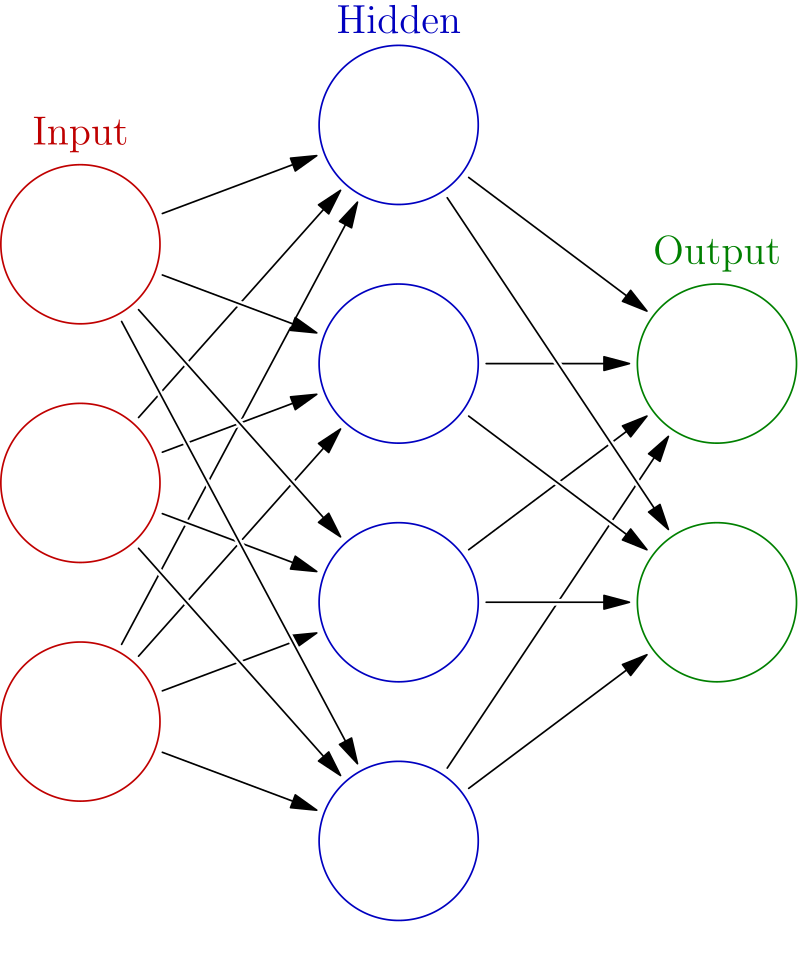
\includegraphics[width=6cm]{img/NN.png}
  \caption{Priklad neuronovej siete}
  \label{vzhladobr}
\end{figure}
\section{RANSAC}
\subsection{Overview}
RANSAC je algoritmus vytvorený Fischlerom a Bollesom, určuje všeobecný prístup k odhadu parametrov, s veľkym podielom outliers v stupnom datasete. Na rozdiel od iných výkonných algoritmov odhadu, ako napríklad M-estimators a meródov najmenších štvorcov s prepojením na strojové učenie. RANSAC bol vytváraný komunitov ľudi používajúci strojové učenie. RANSAC je vzorkovacia technika ktorá generuje kandidáta na minimalny pocet pozorovani potrebnych na zistenie odhadu parametrov leziacich pod modelom. Narozdiel od ostatných vzorkovacích algoritmov, ktoré používaju čo najviac bodov ako môžu, RANSAC používa najmenši počet bodov ako môže.
\subsection{Algoritmus}
\begin{enumerate}
    \item Vybranie minimum náhodných bodov potrebných na určenie parametrov modelu
    \item Vyriešenie parametrov pre model
    \item Určenie koľko bodov z množiny všetkých bodov leží s preddefinovanou \epsilon.
    \item Ak zlomok bodov ležiacich v preddefinovanej ε, presahuje preddefinovaný prah \tau, prehodnotí parametre modelu použitím všetkých identifikovaných inliers a ukonči.
    \item Inak, opakuj kroky 1 až 4, s maximálnym N opakovaniami.
\end{enumerate}
\begin{figure}[!htbp]
  \centering
  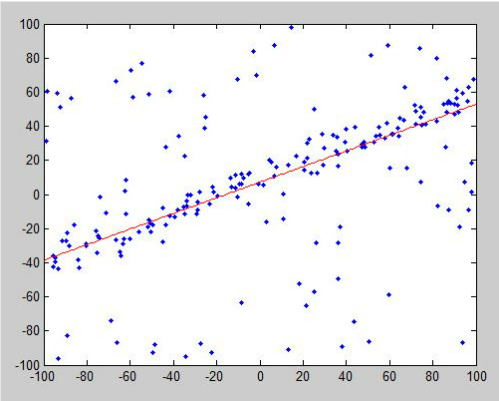
\includegraphics[width=8cm]{img/ransac2D.png}
  \caption{Priklad algoritmu v 2D rovine}
  \label{vzhladobr}
\end{figure}
Modre sú body z datasetu, pomocou RANSAC algoritmu sa určili 2 body, ktoré majú vo svojom subsete najmenej bodov ležiacich mimo alfy.
\subsection{RANSAC 3D}
Podobne ako pri opise vyššie RANSAC 3D funguje s výberom náhodnych troch bodov na ktorých zostaví rovinu a spočita body ležiace v rovine a body ležiace mimo roviny. Algoritmus sa opakuje n-opakovaní a výstupom je najlepší model.
\subsection{Neural guided RANSAC}
\section{KINECT}
Kinect je vstupné zariadenie snímajuce pohyb, vyrobené Microsoftom. Zariadnei obsahuje RGB kamery a infračervený projektor a detektor ktorý monitoruje hĺbku priestoru na zaklade štrukturovateľného svetla alebo na zaklade času trvajúcemu svetlu dopadnuť na objekt, vďaka ktorému vie kinect poskytnúť rekognizáciu giest v reálnom čase. Kinect sa použiva hlavne v hernom priemysle, ale používa sa taktiež na komerčné a akademické učely pretože poskytuje mapovanie priestoru a je lacnejši než profesionálne zariadenia.  
\subsection{Ako funguje}
Infračervený projektor na kinevte posiela modulované infračervené svetlo ktoré je zachytené sensormy. Infračervené svetlo ktoré sa odrazí od bližších objektov ma kratší čas letu ako svetlo ktoré sa odrazí od vzdialenejších objektov, takže sensor sníma ako vymodulovaný vzor bol deformovaný z času letu svetla, pixel po pixeli. Čas príletu meranej hlbky touto metódov môže byť presnejšie vypočítany v kratšom čase, čo zabezpečí viac snímkov za sekundu. Hneď ako kinect naskenuje hlbkovú fotografiu, použije metódu zisťovania hrán k vytýčeniu bližších objektov z pozadia fotky. 
\subsection{Výstup z KINECTU}
Na získanie výstupu z Kinectu je potrebné si nainštalovať Open-source knižnicu LibFreenect2, ktorá je určená na získavanie videi z Kinectu verzie 2. Knižnica disponuje vzorovým kódom, ktorý po spustení zapne Viewer a okno rozdelí na štyri časti a v nich uvidíme výstupy Infra Red kamery, farebnej kamery a depth kamery. Nato aby sme knižnicu mohli používať potrebovali sme doinštalovať potrebné knižnice a súčasti. Na získanie snímky z Kinectu sme použili Python script, ktorý nám vytvorí point cloud súbor,v ktorom budeme hľadať požadovane tvary. 
\subsubsection{List potrebných Knižnic pre Ubuntu 22.04 LTS}
\begin{itemize}
    \item libusb 
    \item TurboJPEG
    \item OpenGL
    \item OpenCL (optional) 
    \item CUDA (optional, NVIDIA only)
    \item VAAPI (optional)
    \item OpenNI2
\end{itemize}
\subsection{Python script}
Z githubu si cloneme freenect2-python, ktorý obsahuje scripty pomocov ktorých vieme získať snímky z Kinectu. Script dump-pcd.py nám vytvorí 2 point cloudy. Po menšej úprave v kóde výstpom je jeden Point cloud a snímka priestoru.
\begin{figure}[!htbp]
  \centering
  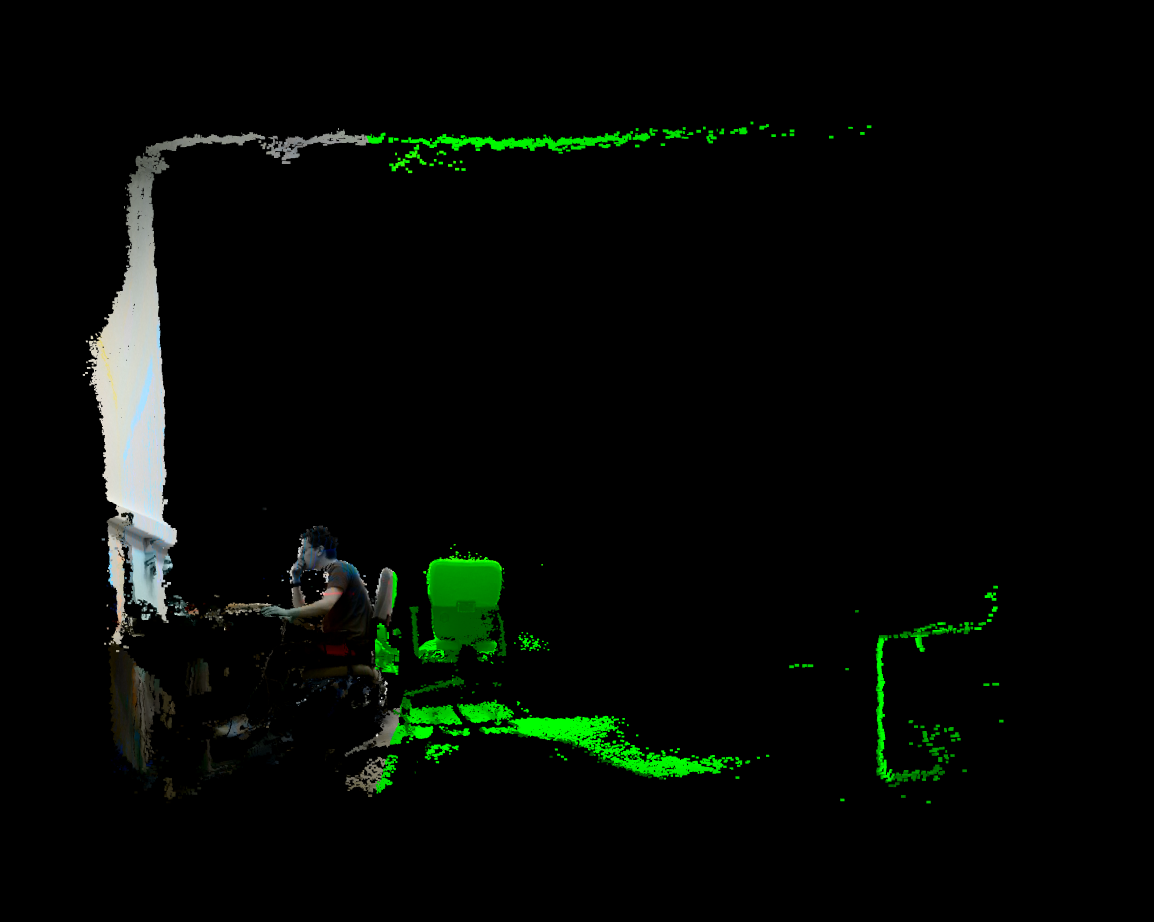
\includegraphics[width=10cm]{img/output_kinect.png}
  \caption{Výstupný Point Cloud z Kinectu}
  \label{vzhladobr}
\end{figure}
\section{Implementavanie RANSAC algoritmu}
\section{Vystupy}
\section{Implementovanie RANSAC alfgoritmu s pouzitim NN}
\section{Kod}

\begin{lstlisting}[
  caption={Vytvorenie PCD pomocou Kinectu},
  label={lst:dump_pcd-py},
  language=python
]
from freenect2 import Device, FrameType
import numpy as np

# Open the default device and capture a color and depth frame.
device = Device()
frames = {}
with device.running():
    for type_, frame in device:
        frames[type_] = frame
        if FrameType.Color in frames and FrameType.Depth in frames:
            break

# Use the factory calibration to undistort the depth frame and register the RGB
# frame onto it.
rgb, depth = frames[FrameType.Color], frames[FrameType.Depth]
undistorted, registered, big_depth = device.registration.apply(
    rgb, depth, with_big_depth=True)

# Combine the depth and RGB data together into a single point cloud.
with open('output.pcd', 'wb') as fobj:
    device.registration.write_pcd(fobj, undistorted, registered)

with open('output_big.pcd', 'wb') as fobj:
   device.registration.write_big_pcd(fobj, big_depth, rgb)
\end{lstlisting}